% Diagrama de atividades da metodologia (UML).
% Compilar isoladamente: pdflatex diagrama-atividade-metodologia.tex
% O PDF gerado é incluído em 2-textuais/metodologia.tex.
\documentclass[tikz,border=4pt]{standalone}
\usepackage[T1]{fontenc}
\usepackage[utf8]{inputenc}
\usepackage{mathptmx}
\usetikzlibrary{positioning,shapes.geometric,arrows.meta,calc}

\begin{document}
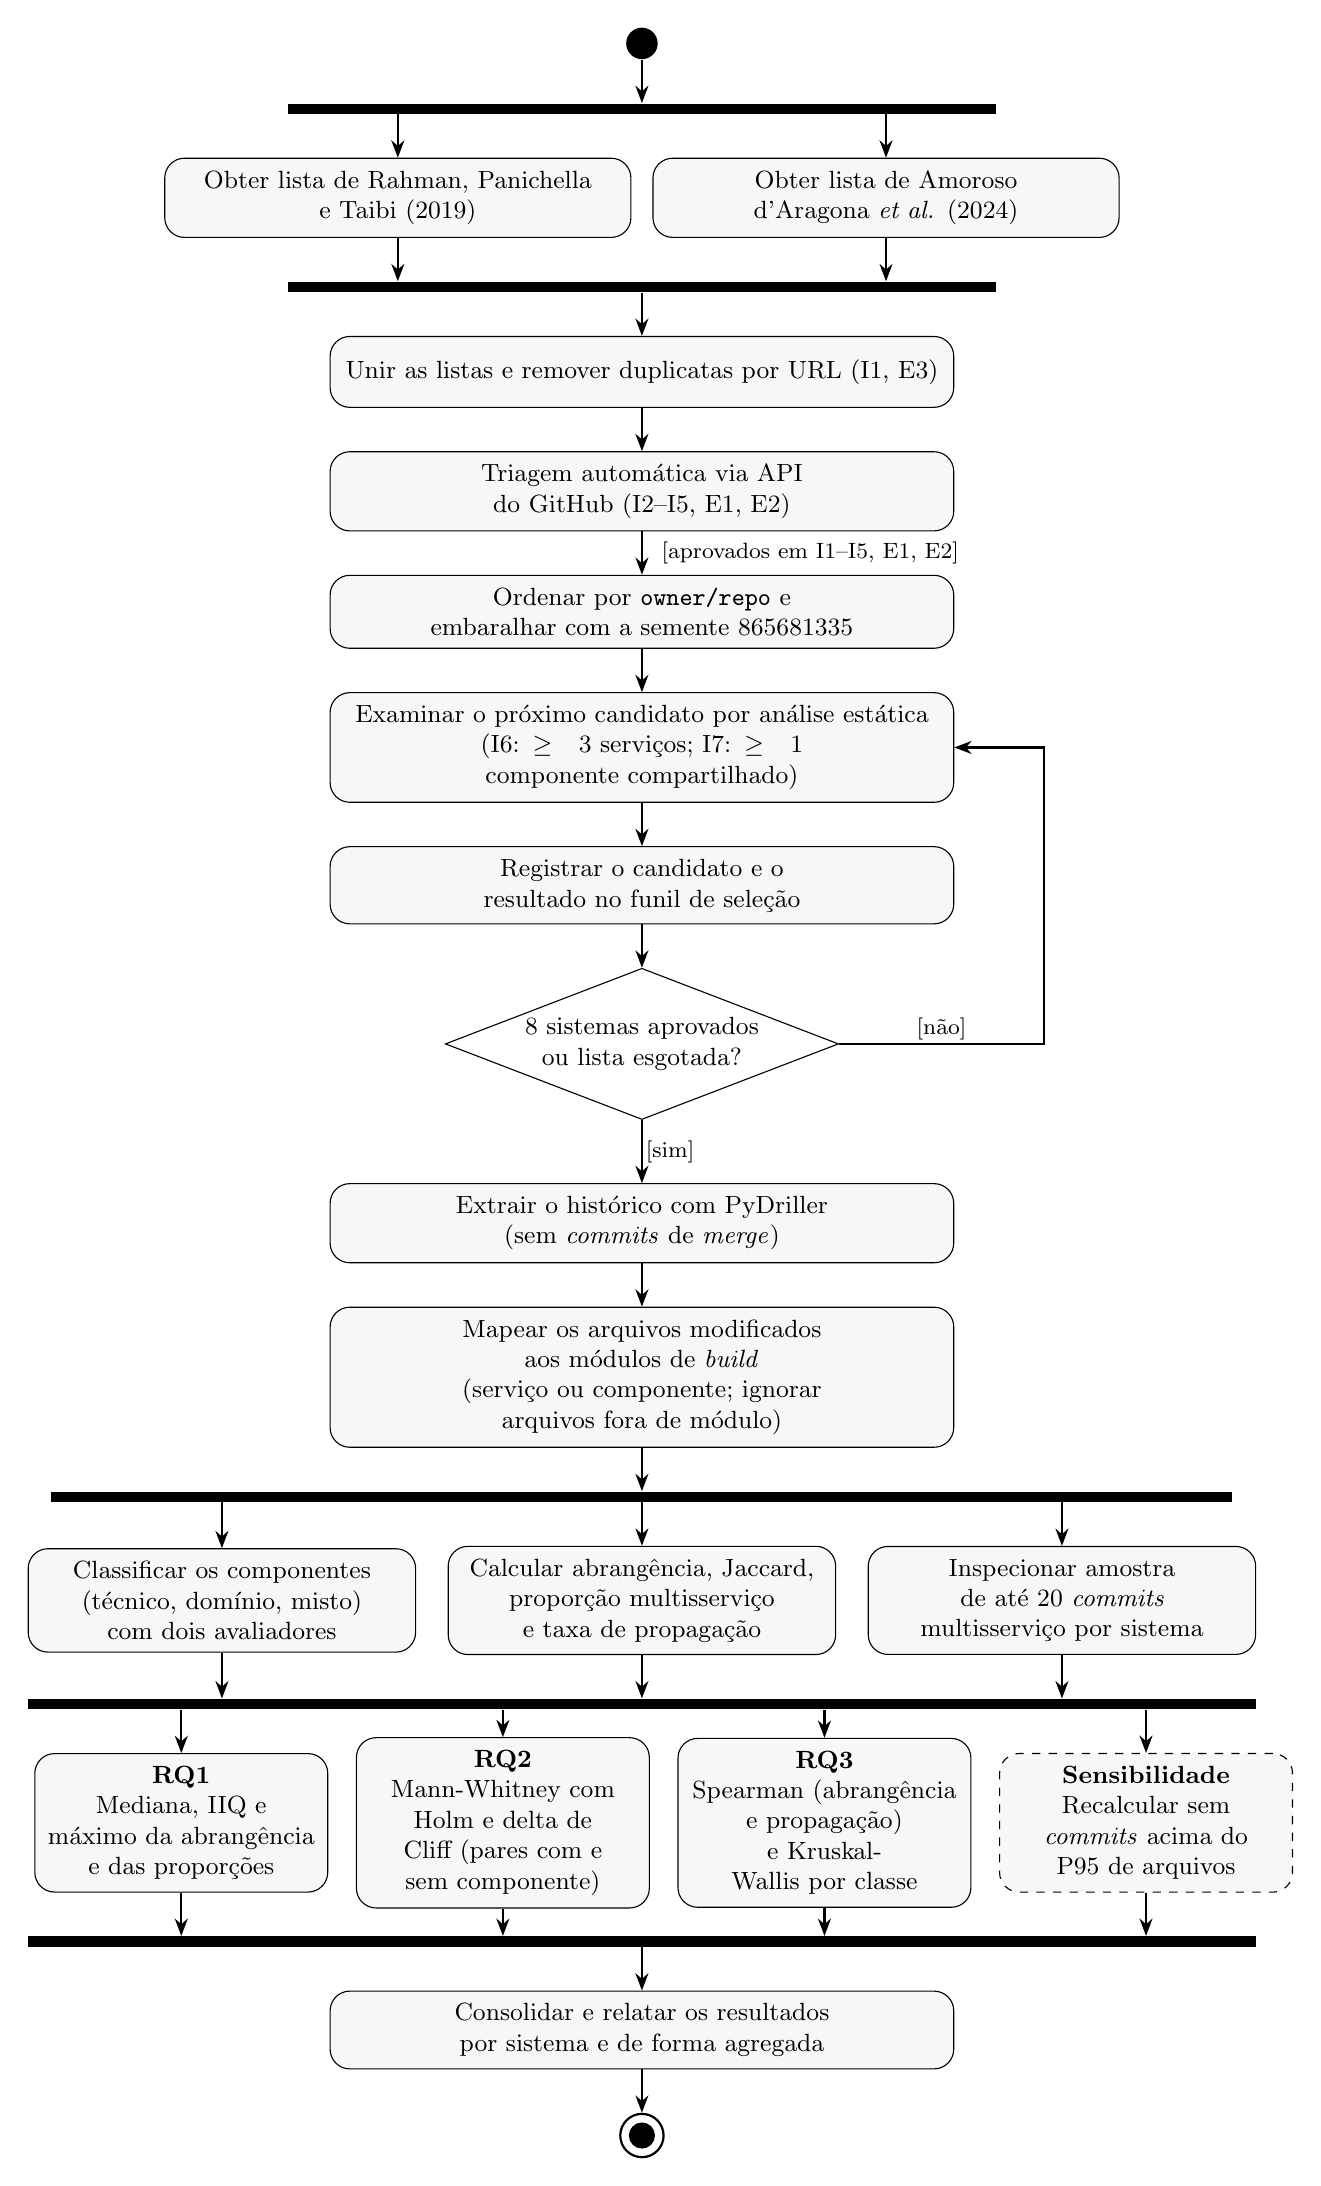
\begin{tikzpicture}[
  font=\small,
  execute at begin node={\hyphenpenalty=10000\relax},
  >={Stealth[length=2.2mm]},
  node distance=5.5mm,
  act/.style={draw, rounded corners=2.5mm, align=center, minimum height=9mm,
              text width=#1, inner sep=1.6mm, fill=gray!6},
  act/.default=7.6cm,
  dec/.style={draw, diamond, aspect=2.6, align=center, inner sep=0.4mm, fill=white},
  bar/.style={fill=black, minimum height=1.3mm, inner sep=0, minimum width=#1},
  bar/.default=12cm,
  guard/.style={font=\footnotesize, fill=white, inner sep=1pt},
  flow/.style={->, thick},
]

% Início
\node[circle, fill=black, minimum size=4mm] (ini) {};

% Seleção do corpus
\node[bar=9cm, below=of ini] (f1) {};
\node[act=5.6cm, below=of f1, xshift=-3.1cm] (rah) {Obter lista de Rahman, Panichella\\e Taibi (2019)};
\node[act=5.6cm, below=of f1, xshift= 3.1cm] (ara) {Obter lista de Amoroso\\d'Aragona \textit{et al.} (2024)};
\node[bar=9cm, below=of rah, xshift=3.1cm] (j1) {};
\node[act, below=of j1] (uni) {Unir as listas e remover duplicatas por URL (I1, E3)};
\node[act, below=of uni] (tri) {Triagem automática via API do GitHub (I2--I5, E1, E2)};
\node[act, below=of tri] (emb) {Ordenar por \texttt{owner/repo} e embaralhar com a semente 865681335};
\node[act, below=of emb] (exa) {Examinar o próximo candidato por análise estática\\(I6: $\geq 3$ serviços; I7: $\geq 1$ componente compartilhado)};
\node[act, below=of exa] (fun) {Registrar o candidato e o resultado no funil de seleção};
\node[dec, below=of fun] (d1) {8 sistemas aprovados\\ou lista esgotada?};

% Coleta
\node[act, below=8mm of d1] (pyd) {Extrair o histórico com PyDriller\\(sem \textit{commits} de \textit{merge})};
\node[act, below=of pyd] (map) {Mapear os arquivos modificados aos módulos de \textit{build}\\(serviço ou componente; ignorar arquivos fora de módulo)};

% Atividades paralelas
\node[bar=15cm, below=of map] (f2) {};
\node[act=4.6cm, below=of f2] (met) {Calcular abrangência, Jaccard, proporção multisserviço e taxa de propagação};
\node[act=4.6cm, left=4mm of met] (cla) {Classificar os componentes (técnico, domínio, misto) com dois avaliadores};
\node[act=4.6cm, right=4mm of met] (amo) {Inspecionar amostra de até 20 \textit{commits} multisserviço por sistema};
\node[bar=15.6cm, below=of met] (j2) {}; % junção das atividades paralelas e bifurcação das análises

% Análises
\node[act=3.4cm, below=of j2, xshift=-5.85cm, minimum height=17mm] (rq1) {\textbf{RQ1}\\Mediana, IIQ e máximo da abrangência e das proporções};
\node[act=3.4cm, right=3.5mm of rq1, minimum height=17mm] (rq2) {\textbf{RQ2}\\Mann-Whitney com Holm e delta de Cliff (pares com e sem componente)};
\node[act=3.4cm, right=3.5mm of rq2, minimum height=17mm] (rq3) {\textbf{RQ3}\\Spearman (abrangência e propagação) e Kruskal-Wallis por classe};
\node[act=3.4cm, right=3.5mm of rq3, minimum height=17mm, dashed] (sen) {\textbf{Sensibilidade}\\Recalcular sem \textit{commits} acima do P95 de arquivos};
\node[bar=15.6cm, below=of rq1, xshift=5.85cm] (j3) {};
\node[act, below=of j3] (con) {Consolidar e relatar os resultados por sistema e de forma agregada};

% Fim
\node[circle, draw, thick, minimum size=5.5mm, below=of con] (fim) {};
\node[circle, fill=black, minimum size=3.3mm] at (fim) {};

% Fluxos
\draw[flow] (ini) -- (f1);
\draw[flow] (f1.south -| rah) -- (rah);
\draw[flow] (f1.south -| ara) -- (ara);
\draw[flow] (rah) -- (j1.north -| rah);
\draw[flow] (ara) -- (j1.north -| ara);
\draw[flow] (j1) -- (uni);
\draw[flow] (uni) -- (tri);
\draw[flow] (tri) -- node[guard, right=2mm] {[aprovados em I1--I5, E1, E2]} (emb);
\draw[flow] (emb) -- (exa);
\draw[flow] (exa) -- (fun);
\draw[flow] (fun) -- (d1);
\draw[flow] (d1.east) -- node[guard, above] {[não]} ++(2.6cm,0) |- (exa.east);
\draw[flow] (d1) -- node[guard, right] {[sim]} (pyd);
\draw[flow] (pyd) -- (map);
\draw[flow] (map) -- (f2);
\foreach \n in {cla,met,amo}{
  \draw[flow] (f2.south -| \n) -- (\n);
  \draw[flow] (\n) -- (j2.north -| \n);
}
\foreach \n in {rq1,rq2,rq3,sen}{
  \draw[flow] (j2.south -| \n) -- (\n);
  \draw[flow] (\n) -- (j3.north -| \n);
}
\draw[flow] (j3) -- (con);
\draw[flow] (con) -- (fim);

\end{tikzpicture}
\end{document}
